
\chapter{Glyph-based Visual Compression of Time Series Visualizations}
\label{chap:timeseries}

\begin{chapquote}{John F. Kennedy}{``We must use time as a tool, not as a crutch.''}
\end{chapquote}
%Time is what we want most, but what we use worst.

\section{Introduction}
In many applications, such as finance, meteorology, biology, chemistry, physics, and engineering, users have collected a large volume of time series data.
A collection of time series that record phenomena of a similar nature is defined as a \emph{time series corpus} $\mathcal{T}$.
On one hand, users often find that it is time consuming and cognitively demanding to browse many time series in a time series corpus.
On the other hand, the corpus provides an opportunity to identify frequently occurring patterns.
When such patterns are of a reasonable length, it is advantageous to replace them with a short abstract representation, such as a text label, a signature pattern, a glyph or a combination of these (\eg, \cite{haovisual2012}).
This is a form of \emph{visual compression}, which is commonly seen in real life.
For example, in signage management, frequently encountered restrictions and events are encoded as signs and icons, while those of an occasional or exceptional nature are written in text. From an information-theoretic perspective, such a strategy is fundamentally the same as that used in entropy encoding and dictionary encoding \cite{Chen10,lang2010}.

In time series processing and visualization, the algorithm for identifying \emph{Frequent Long Patterns} (FLPs) plays a critical role.
It has to be sufficiently tolerant to noise that causes variations to patterns in the corpus.
Without a high-degree of noise tolerance, the criteria of \emph{frequent} and \emph{long} could not be met, and the objective of visual compression could not be fulfilled.
However, paradoxically the FLP algorithm is also required to exclude any anomalous patterns, which would easily be mistaken as frequently occurring patterns once they are visually compressed.
In many situations, an anomalous pattern differs from frequent occurring patterns in a subtle way, and a conventional FLP algorithm may not handle the features that characterise such differences.

\begin{figure}[t!]
\centering
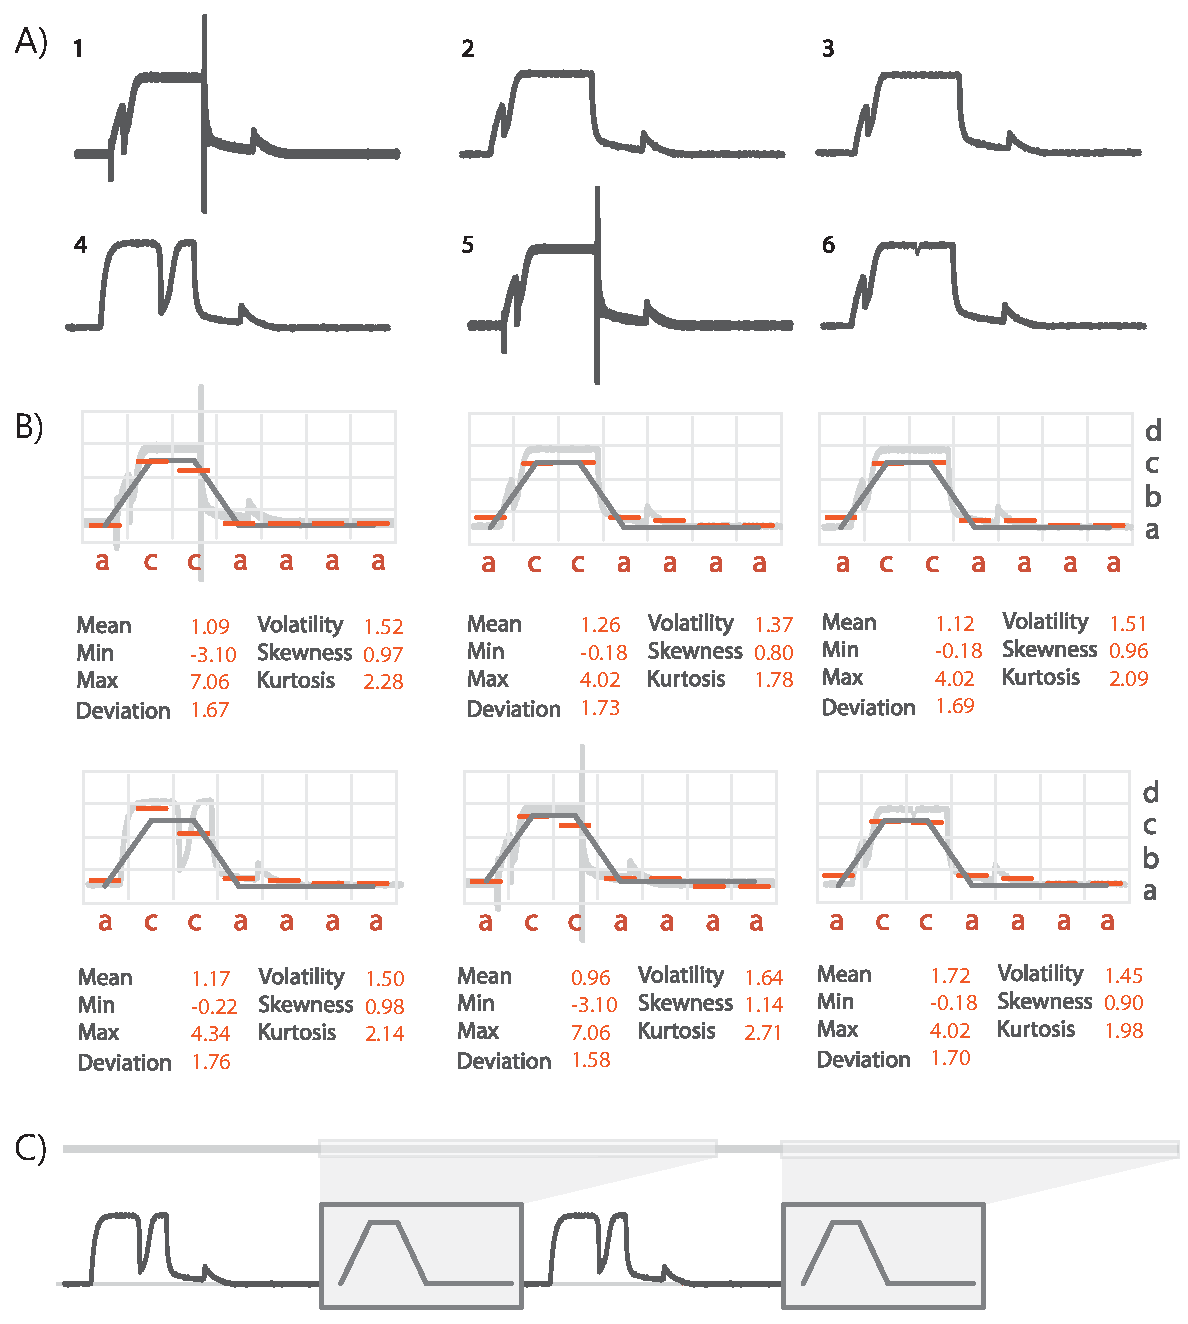
\includegraphics[width=.6\textwidth]{images/timeseries/ecg_bad_refine}
\caption{A) Six time series subsections identified in a time series corpus of space shuttle valve time function taken from \cite{keogh_datasets}.
B) Symbolic representation of each time results in all motifs being seen as the same, however their more detailed metrics/features differ.
C) Leaving out the anomalous pattern (A4) from the compression as requested by a user means that the final time series compresses the actual common motifs and leaves the anomalous pattern in plain view.}
\label{fig:bad_example}
\vspace{-10pt}
\end{figure}

Figure \ref{fig:bad_example} A) shows six segments of a time series.
They all appear to be fairly similar, and a typical FLP algorithm (Figure \ref{fig:bad_example} B)) would consider them to be the same.
However, the 4th segment is an anomaly.
An ideal visual compression should not replace this segment with a glyph, while compressing as many others as possible, as illustrated in Figure \ref{fig:bad_example} C).

This chapter presents two major contributions.

The first is a new algorithm for detection of frequent long patterns in time series data.
This algorithm extends on existing techniques to detect FLPs in a time series corpus.
 
Secondly, we present a visual analytics approach to address the paradoxical conflict of requirements upon an FLP algorithm.
Consider that an FLP identified by an FLP algorithm is a model. The basic idea is to add an additional filtering capability to this model. As the filtering does not take place within the parameter space of the original FLP algorithm, it can handle features that the FLP algorithm cannot. The function of visual analytics is to support the following in an iterative manner:

%
\begin{enumerate}
\item discovery of any anomalous patterns that may have been included by an FLP model;
\item compute a bag of features that may be used to characterise different time series segments identified by an FLP model, and to visualise them in the feature space;
\item assist users in a number of analytical tasks for identifying the appropriate filters, \eg, results clustering and tagging, and observing the effects of feature selection on filtering results; and
\item facilitate model editing by transforming interaction in visualization to text-based instructions in the FLP model.
\end{enumerate}

Having created a glyph dictionary represent the frequent long patterns, these glyphs can be used for glyph-based compression of time series visualizations.\\

In the remainder of this chapter, we first give a brief overview of time series analysis and visualization in Section \ref{sec:related_work}.
In Section \ref{sec:va-approach} we outline a visual analytics loop for analysing, visualising, testing, and editing an FLP model, and we describe a prototype system that supports such a visual analytics loop.
In Section \ref{sec:flp_detection_model}, we describe an FLP algorithm that serves as the core component of an FLP model.
In Section \ref{sec:feature_space}, we describe a collection of features that have been implemented to support model analysis and editing.
In Section \ref{sec:model_editing} we describe the model editing system and introduce the logical operators that can be used to combine models as well as build up rules for parameter refinement. Finally, in Section \ref{sec:vis_results} we present a visualization to render the results of the time series compression. 

%=====================
\section{Related Work}
\label{sec:related_work}

The related work can be divided in to: \emph{time series analysis}, focusing specifically on normalisation, approximation, and similarity; and \emph{time series visualizations}.

\subsection{Time Series Analysis}
\label{sec:time_analysis}
Time series analysis encompasses five main sub-categories of operations: indexing, clustering, classification, summarisation, and anomaly detection \cite{lina2003}. 

\begin{enumerate}
\item \textbf{Indexing} to store, search and retrieve time series data in a data repository.\\
\item \textbf{Clustering} to group a set of time series by their similarity. \\
\item \textbf{Classification} to determine if a new time series belongs to a specific pre-defined class.\\ 
\item \textbf{Summarization} provides a compact representation of a time series and/or its main attributes (\eg, a feature vector or a visualization). \\
\item \textbf{Anomaly detection} can highlight anomalous incidents based on the profiles of a set of normal events.\\
\end{enumerate}

For all of the above tasks, computing the similarity between time series data is a common task.
However, before similarity measures can be used, preprocessing steps often need to be carried out first.
This includes normalising the data (so that data is comparable in terms of its range), then approximating it (to make it the series amenable to similarity measures).
Here we document the approaches used to perform all three steps.

%%Discrete vs continuos time?
%%Normalisation?

\noindent\textbf{Normalization.}
Before comparing two or more time series, an adjustment may need to be made to the data sets so that the data itself is comparable.
For example, if we are looking for commonality in trends, the similarity score should be comparing the overall topology between points, rise and falls, rather than being too concerned with where on the \emph{y}-axis those trends reside.
This step is called normalisation.
One common approach is Z-normalisation, where the time series are manipulated to have a mean of zero and a standard deviation of one. 

% \noindent The lower bounding condition is formulated as:
% \begin{equation}
% D_{feature}(T(X),T(Y)) \; \leq \; D_{object}(X,Y) 
% \label{eq:bounding}
% \end{equation}
% where $D_{feature}$ is the distance between objects in feature space (Agrawal et al used the Euclidean distance), $T$ is the transform function from object space to feature space (DFT) and $D_{object}$ is the real distance between objects $X$ and $Y$ (the Euclidean distance again). 
% http://csdl-techreports.googlecode.com/svn-history/r511/trunk/techreports/09-08/bounding.tex

\noindent\textbf{Approximation.}
%
\begin{figure}[ht!]
\centering
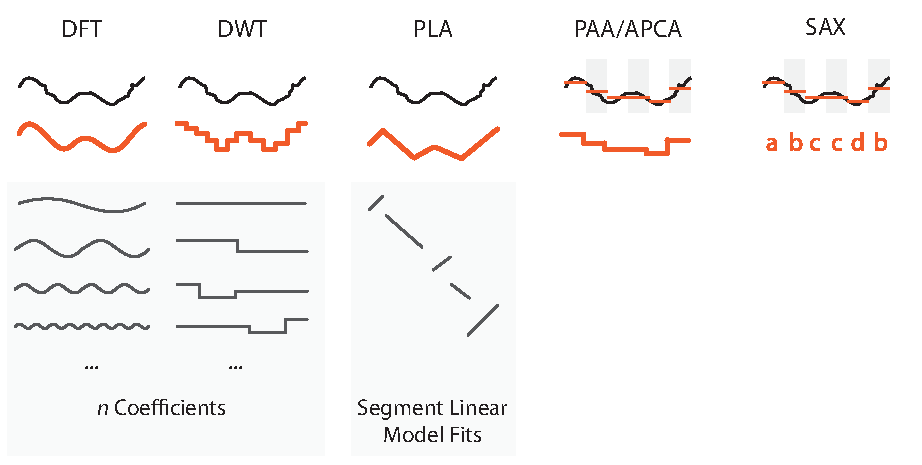
\includegraphics[width=.7\textwidth]{images/timeseries/approximations.pdf}
\caption{Common representations of a time series with Discrete Fourier Transforms (DFT), Discrete Wavelet Transforms/Haar Wavelet (DWT), Piece-wise Linear Approximation (PLA), Piece-wise Aggregation Approximation and Adaptive Piece-wise Constant Approximation (PAA/APCA) and Symbolic Aggregate Approximation (SAX).}
\label{fig:approximation}
\vspace{-10pt}
\end{figure}
%
Following normalisation, we may wish to reduce the dimensionality of the data. 
This means that instead of comparing a time series in terms of real data points, we compare approximations that are smaller in size but retain the important features of the series. 
There are numerous techniques available for this process, all with their own limitations and strengths. 
Figure \ref{fig:approximation} shows the most relevant and commonly used techniques for time-series approximation, including: 

\begin{enumerate}
\item \textbf{Discrete Fourier Transformation (DFT)} \cite{faloutsos1994fast} is an algorithm capable of representing the overall features of a time series through spectral decomposition.
This means that the signal represented by the time series is decomposed into a series of sine (and/or cosine) waves each represented by a Fourier coefficient \cite{keogh2001dimensionality} - this proves to be a very efficient way of compressing data; 

\item \textbf{Discrete Wavelet Transformation (DWT)} \cite{chanefficient1999} is an algorithm similar in principle to DFT, however it has one key difference in that some of the wavelet coefficients represent small local regions of the series meaning that wavelets lend themselves to providing a multi-resolution view of a time series.
The results of DWT do not lend themselves to being indexed (for comparison purposes).
However an extension called the Haar Wavelet can be calculated efficiently and its outputs can be indexed for efficient time series matching \cite{chanefficient1999}.
The key drawback with DWT is that the length of the time series must be an integral power of two \cite{keogh2001dimensionality}; 

\item \textbf{Piecewise Linear Approximation (PLA)} \cite{cameron1966piece} or Segmented Regression is an algorithm that breaks a time series up in to `windows'.
Each window is then represented with a line segment that best fits the values in that window;

\item \textbf{Piecewise Aggregate Approximation (PAA)} \cite{keogh2001dimensionality} works similar to PLA, however instead of creating a line of best fit across the points, PAA simply stores the average value of time points within each window.
The approach is simple yet is shown to rival DFT and DWT \cite{lina2003,keogh2003need}; 

\item \textbf{Adaptive Piecewise Constant Approximation (APCA)} \cite{keogh2001locally} is algorithmically similar to PAA with extensions that further compress the representation using a technique common to data compression known as run-length encoding (RLE).
This extension is the addition of a second number beside the mean value of the window indicating the length of the segment; and 

\item \textbf{Symbolic Aggregate Approximation (SAX)} \cite{lina2003,linexperiencing2007}, illustrated in Figure \ref{fig:approximation-sax}, which builds on PAA to take the average values calculated for each window then assigns a letter to that window based on where the mean value falls under a Gaussian curve.
The result, as illustrated in Figure \ref{fig:approximation-sax} is a symbolic representation of a time series that lends itself to many computational manipulations such as hashing or storage in data structures such as suffix trees for fast pattern searching.
Suffix trees have been used by Lin \etal \cite{lina2003}, to build a motif discovery tool for time series data, capable of highlighting anomalous data.
A weakness of the symbolic approach however is the need to define a window and alphabet size ahead of time - these will differ depending on the domain due to differences in periodicity, variance for example.

\end{enumerate}

\begin{figure}[b!]
\centering
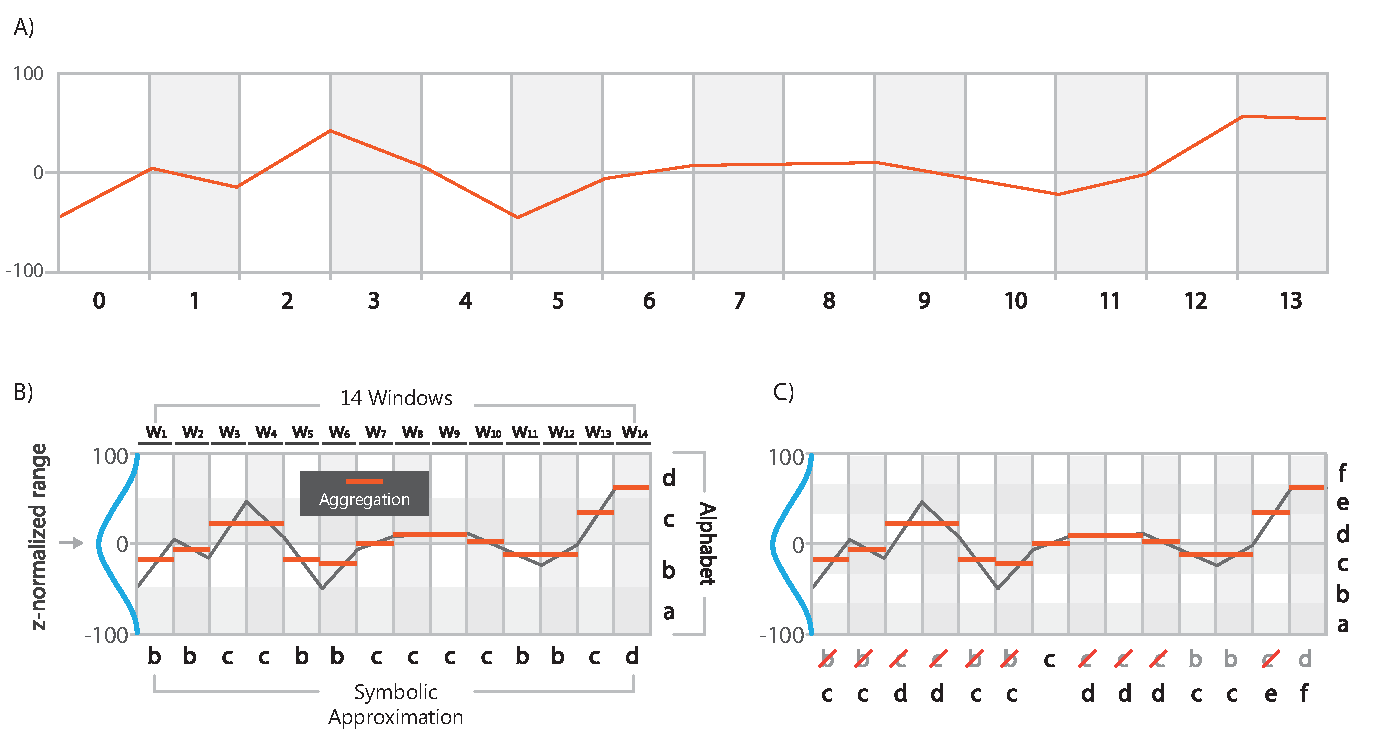
\includegraphics[width=\textwidth]{images/timeseries/approximation-sax-horizontal}
\caption{A) A general time series.
B) The symbolic approximation algorithm (see Section \ref{sec:time_analysis}) is applied.
Normalization is performed (blue line) giving a mean of zero and standard deviation of one.
Then, given a window of two, PAA is applied to find the average between the two values.
This normalised average is then assigned a letter based where in the Guassian distribution the average falls.
C) An increase in alphabet size increases the granularity of the approximation.}
\label{fig:approximation-sax}
\end{figure}

\noindent\textbf{Similarity.}
Following these steps, comparison can be performed on the outputs of the approximation which will give an idea of how close a time series is to another.
Starting with the most simple of methods, there is the Euclidean distance, where for two time series ($t_1, t_2$) the Euclidean distance would be calculated using $\sqrt{\sum_{k=1}^{n}(t_{1_k} - t_{2_k})^2}$ where $t_{n_k}$ represents a point in time series $n$. 
This metric is fast to compute due to its simplicity, however it carries the caveat that the two sequences must be of the same length.
When sequences are not of the same length, there are more complicated algorithms largely based on dynamic programming methodologies including:
\begin{enumerate}
\item \textbf{Dynamic Time Warping} \cite{berndt1994using} allows for comparison between sequences of varying lengths and also support shifts in the series; 
\item \textbf{Edit distance with Real Penalty (ERP)} allows for gaps in a time series that may be penalised using some configurable value;
\item \textbf{Longest Common Subsequence (LCSS)} \cite{vlachos2003indexing} introduces a threshold value allowing a degree of mismatch between sequences; and 
\item \textbf{Edit Distance on Real sequences (EDR)}  \cite{chen2005robust} merges the concept of gaps and mismatch thresholds presented in ERP, and LCSS respectively.
\end{enumerate}

Due to the use of dynamic programming techniques, DTW, ERP, LCSS, and EDR have limitations in that there are many comparisons made between sequences that have no relevance whatsoever.
To address these limitations, there is the Fast Time Series Evaluation \cite{morse2007efficient} algorithm which introduced a more efficient way of building up the comparison matrix meaning that non-related sequences are never compared.

\subsection{Time Series Visualization}

More complete surveys of time series visualization have been conducted by Silva and Catarci \cite{Silva00} and Aigner \etal \cite{Aigner07}.
TimeViz \footnote{\url{http://survey.timeviz.net/}} accompanies the associated book on ``Visualization of Time Oriented data'' by Aigner \etal \cite{aigner2011visualization} and provides a comprehensive overview of over one hundred time series visualization techniques.
Here we highlight some of the work in the visualization domain that aims to ease the task of time series analysis and provide a more effective means for users to navigate their data.
Such work includes:
\begin{enumerate}
\item \emph{StackZooming} \cite{javedstack2010} which provides a hierarchical zooming interface for time series data;
\item a spectral visualization system for visualising overviews of financial data by Keim \etal \cite{Keim:2006};
\item the use of ``lenses' to focus on particular areas of a time-series by Kincaid \etal \cite{kincaidsignallens:2010} and Zhao \etal \cite{zhaoexploratory2011};
\item \emph{LiveRAC} \cite{mclachlanliverac:2008} for computer/information system management;
\item \emph{Horizon charts} \cite{Heer09} that attempt to aid comparison of many time series in one height fixed display;
\item \emph{TimeSearcher} \cite{hochheiser2001} and \emph{VizTree} \cite{lin2005} that allow for exploration of time series via a visual query interface;
\item spiral visualizations to allow for trend discovery in datasets by Weber \etal \cite{weber2001} and Drocourt \etal \cite{Drocourt11};
\item importance-driven layouts for time series data by Hao \etal \cite{haoimportance-driven2005};
\item multi-resolution techniques for exploration of time-series data from Hao \etal \cite{haomulti-resolution2007}; and
\item the visual exploration of frequent patterns in time series data from Hao \etal \cite{haovisual2012}. 
\end{enumerate}

Glyphs have been used for visualization in time series for a number of tasks.
Many such uses have been in order to summarise a series where examples include those from Keogh \etal with intelligent icons\cite{keoghintelligent2006}, Fuchs \etal \cite{fuchsevaluation2013} Ward and Guo \cite{ward2011}, and Wickham \etal \cite{wickham2012}.
They have also been used to represent uncertainty in time series data by Aigner \etal \cite{aigner05planningLines}. 

\section{A Visual Analytics Approach}
\label{sec:va-approach}

Figure \ref{fig:analytics_environment} shows an overall pipeline for detecting FLPs in a time corpus, and for compressing a time series with glyphs.
Steps 1, 2, 5, and 6 represent the pipelines traditionally used in the literature.
Steps 3 and 4 represent the newly added visual analytics steps for model testing, visualization, analysis, and editing.

Similar to the visual analytics system by Legg \etal \cite{legg13} for sports video search refinement, this system will allow users to refine FLP models resulting from a conventional FLP algorithm so that users may filter the FLPs most appropriate for their use case. 

\begin{figure*}[ht!]
\centering
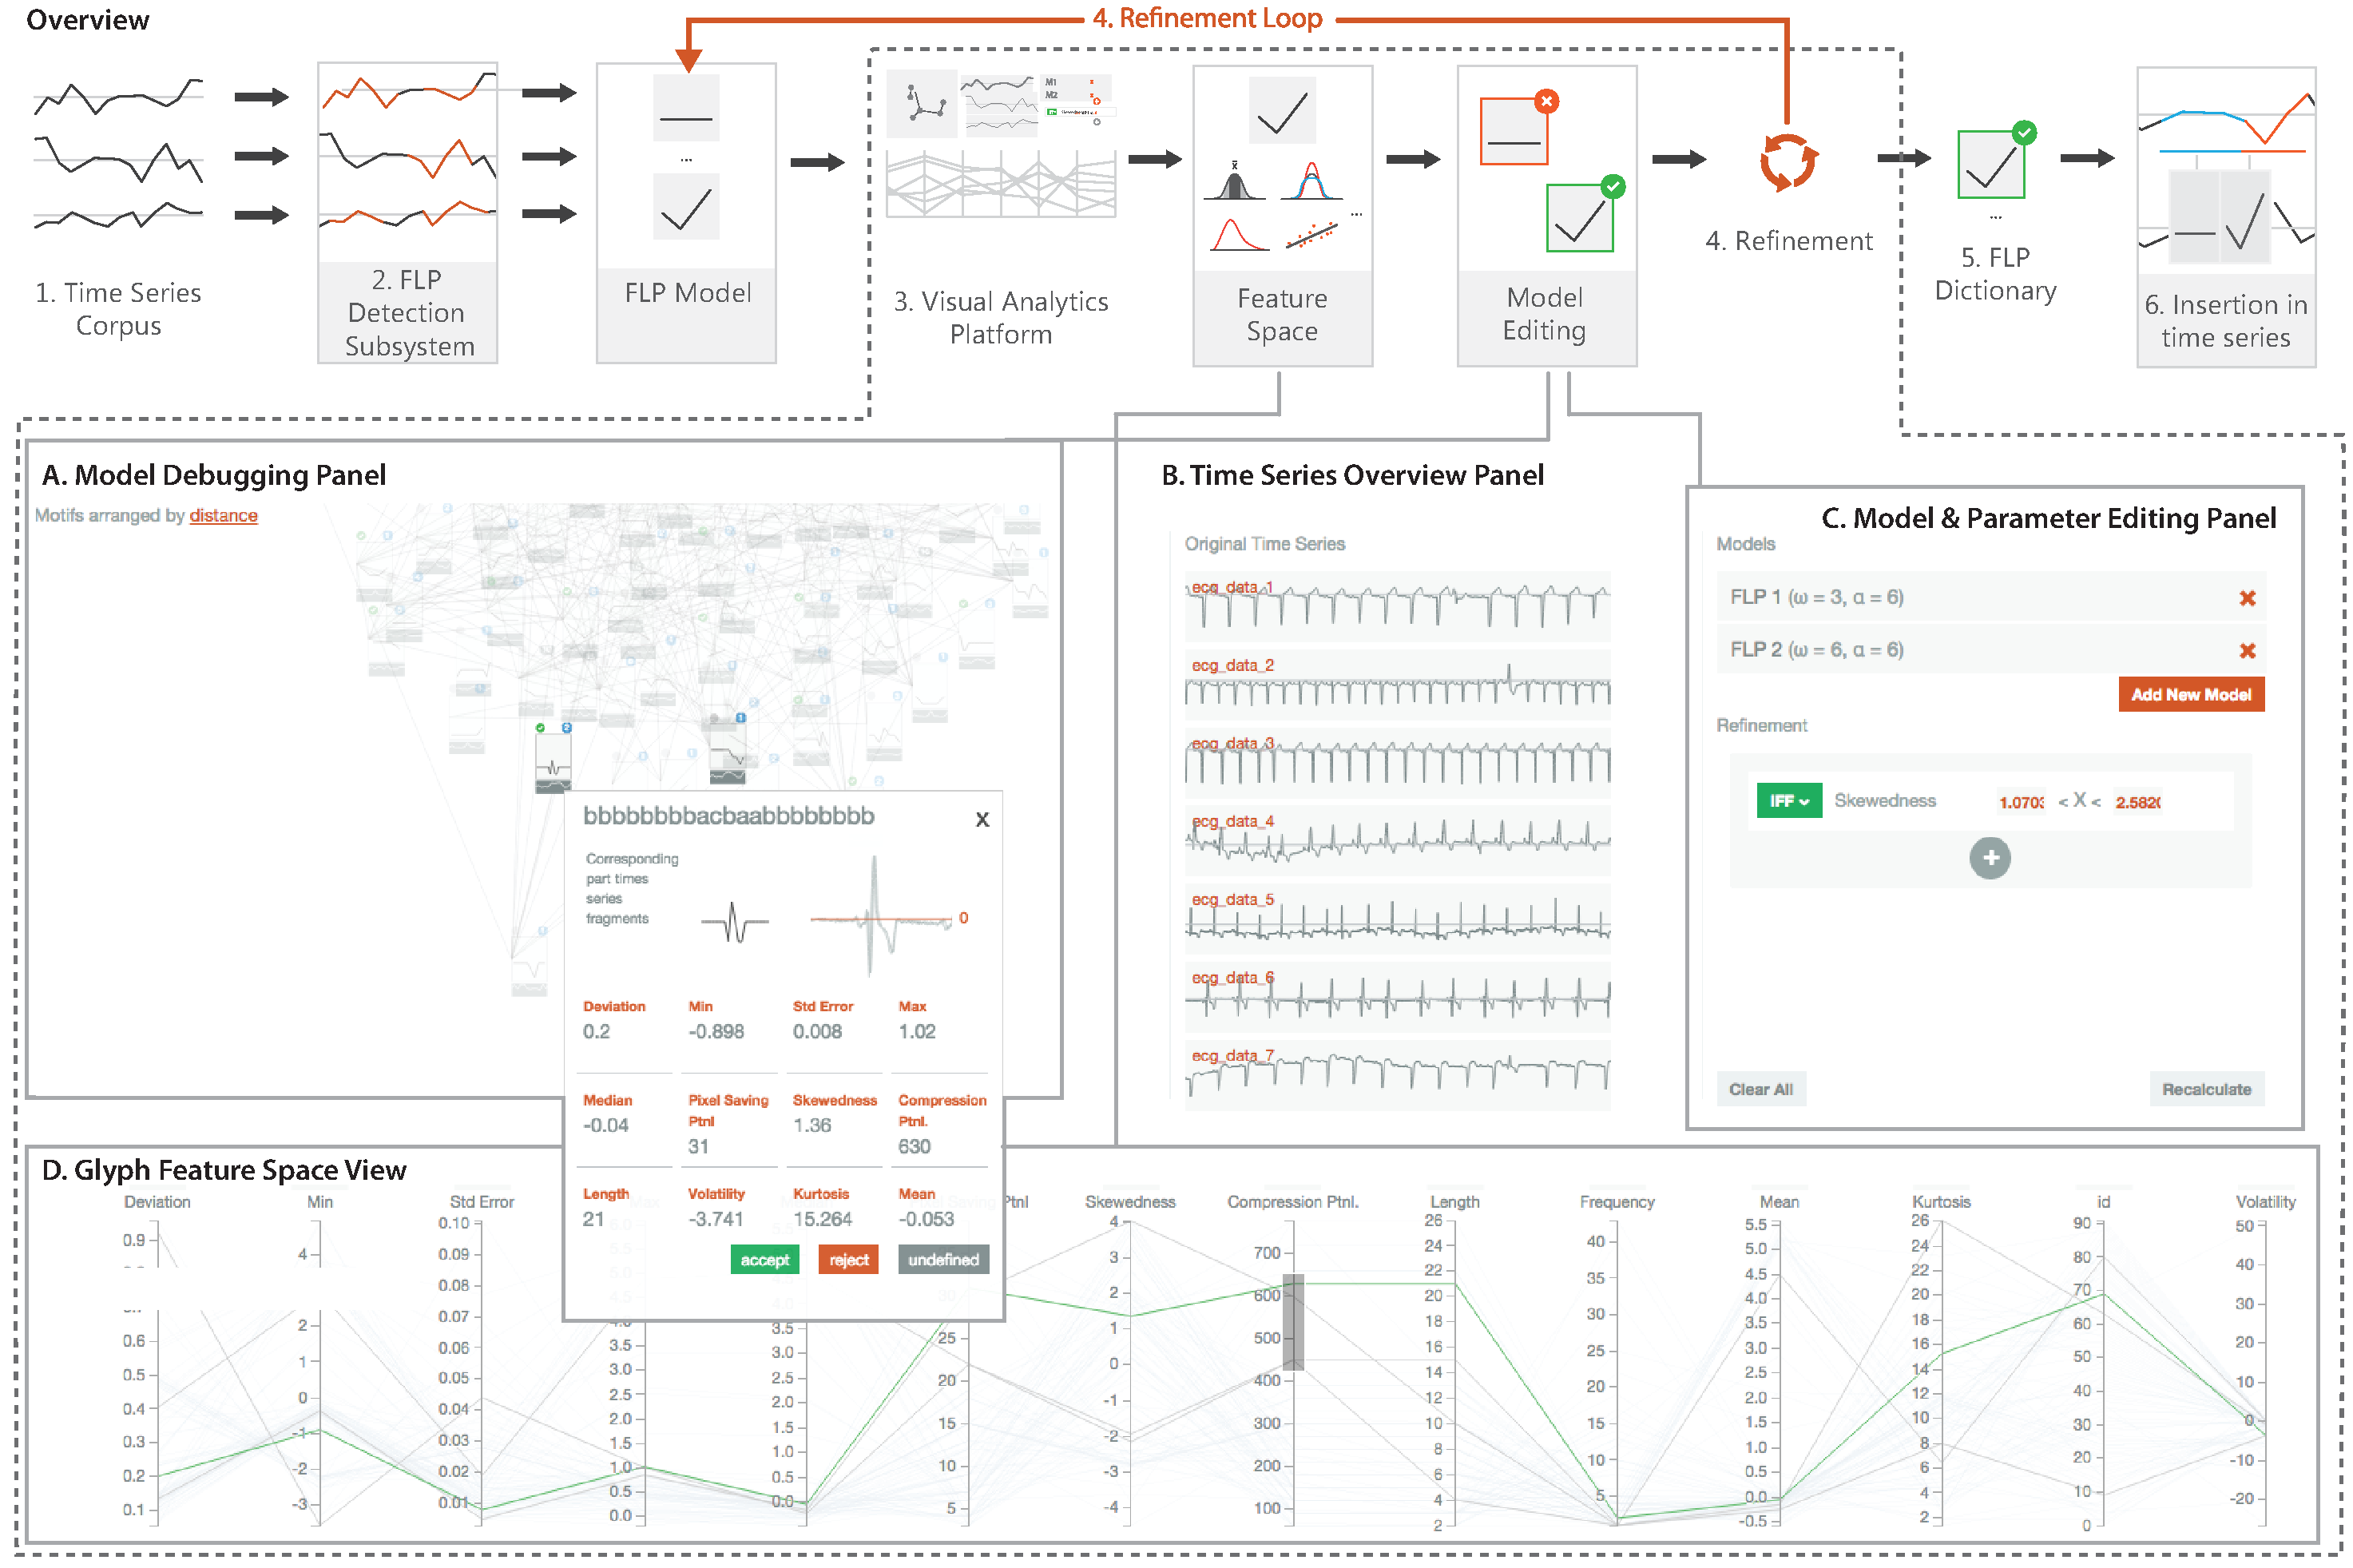
\includegraphics[width=\textwidth]{images/timeseries/application}
\caption{The overview of the process followed in this chapter and a screenshot of the visual analytics platform built to facilitate this process.
The visual analytics platform interface has four interlinked panels to support:
A) visual model debugging;
B) overview of the larger time series to support context views for each motif (where it occurs in the actual time series);
C) model and parameter editing; and
D) navigation and refinement of the feature space for each motif.}
\label{fig:analytics_environment}
\vspace{-10pt}
\end{figure*}

This pipeline is detailed as follows:

\begin{enumerate}
\item a \textbf{Time Series Corpus} as input to the system - this is usually a very large collection of time series. 
\item a \textbf{Frequent Long Pattern (FLP) detection subsystem} - this detects FLPs in the time series, the output of which is a list of different FLP candidates.
A user can choose a specific FLP as an individualised FLP model.
The model will detect only patterns that match this FLP;
\item a \textbf{Visual Analytics Platform} consisting of a number of components to aid model output view, edit, and test and refinement operations.
The interface, shown in Figure \ref{fig:analytics_environment} realises this platform through four interlinked panels:
\begin{itemize}
\item\textbf{A) Model Debugging Panel}:  results from the FLP model are presented in this overview area where results of the model can be approved or rejected. The network view presents each motif as a glyph representing the approximation amongst its feature space. These glyphs can be arranged in a number of different topologies: 
\begin{enumerate}
\item by distance between the symbolic representation of each motif - this is calculated on motifs with equal lengths through their Euclidean distance.
This is defined by the equation below from Lin \etal \cite{linexperiencing2007}

\begin{equation}
MINDIST(S_X,S_Y) = \sqrt{\frac{n}{w}} \sqrt{\sum_{i=1}^{w} (dist)(S_{X_i}, S_{Y_i})^2}
\end{equation}

where the $dist$ function indicates the use of a lookup table to determine the distance between two letters, say A and D in the symbolic approximation. Since A and D are further away from each other than A and B for each, $dist(A,D)$ would return a larger value than $dist(A,B)$

\item by whether motifs have been accepted or not; or 
\item by a hierarchy representing parent-child relationships where parent motifs (\eg, abbaca) have a sequence that contains N child motifs (e.g., abb, bb, bba, or baca)
\end{enumerate}

This view also provides users with a way to select a glyph and view more information about the motif it represents. A popup shown in Figure \ref{fig:node_popup_detail}A allows users to mark motifs as accepted or rejected, view their feature space in more detail, obtain their context in the collection of time series being analysed (see Figure \ref{fig:analytics_environment} B) and view the original time series.

\begin{figure}[t!]
\centering
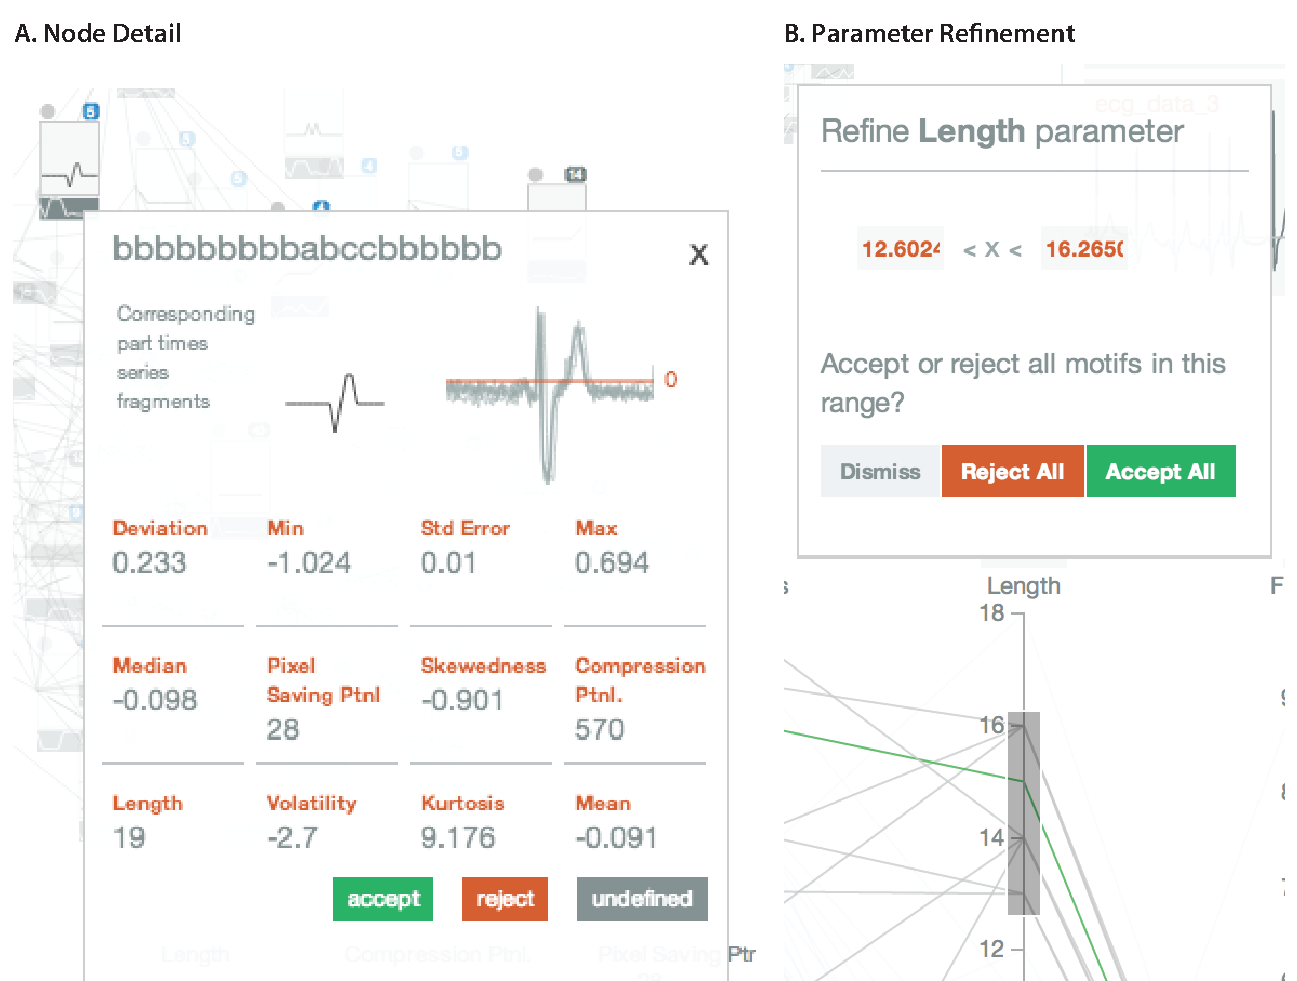
\includegraphics[width=.9\textwidth]{images/timeseries/application_node_popup_zoom}
\caption{A) Node detail view showing the feature space of the nodes, the approximation, and the corresponding parts of the time series that this motif is associated with.
Additionally, the context is shown for the motif in the time series panel on hovering over a node.
B) On brushing an axis in the parallel coordinate plot, a parameter refinement window appears to allow the user to either remove results based on particular parameters or to accept them}
\label{fig:node_popup_detail}
\vspace{-10pt}
\end{figure}
 
\item\textbf{B) Time Series Overview Panel}: provides a summary view of the time series being used by the motif finding algorithm. 
This is also used to highlight where motifs occur within the time series to provide further contextual information to users.

\item\textbf{C) Model and Parameter Editing Panel}: split in to two sections: the \emph{model} area - this area allows users to create new models, changing the window $\omega$ and alphabet size $\alpha$ and combine the results of these models; and the \emph{refinement} area, providing an interface for users to edit the feature ranges required for acceptance or rejection of a motif. These features can be combined with a number of logical operations such as union (OR), intersection (AND) and subtract (SUB). 
Each feature may have a value range that is less than, less than or equal to, greater than or greater than or equal to some limit value.
Recalculation can be performed at any point and results are updated in the network and parallel coordinate views. 
See Section \ref{sec:model_editing}. 

\item\textbf{D) Feature Space Panel}: to visualise the feature space of the motifs, we use parallel coordinate plots. 
Users can brush a combination of axes to find the ``best'' parameters that yield the motifs they really want. 
This is aided by a refinement window shown in \ref{fig:node_popup_detail} B and a link with the network view which filters out nodes that have parameters outside the brushed region(s) (see \ref{fig:analytics_environment} A and D).
See Section \ref{sec:feature_space}.

\end{itemize}

\item a \textbf{Refinement Loop} which allows re-runs of the FLP detection model(s) given user-defined refinements to the conditions required for motif acceptance;
\item a collection of \textbf{Accepted Motifs}; and 
\item a \textbf{Time Series Compression} step which inserts the motifs as glyphs in to time series for compression and/or anomaly detection (see Section \ref{sec:vis_results}).

\end{enumerate}

\section{FLP Detection Subsystem}
\label{sec:flp_detection_model}

\begin{figure*}[ht!]
\centering
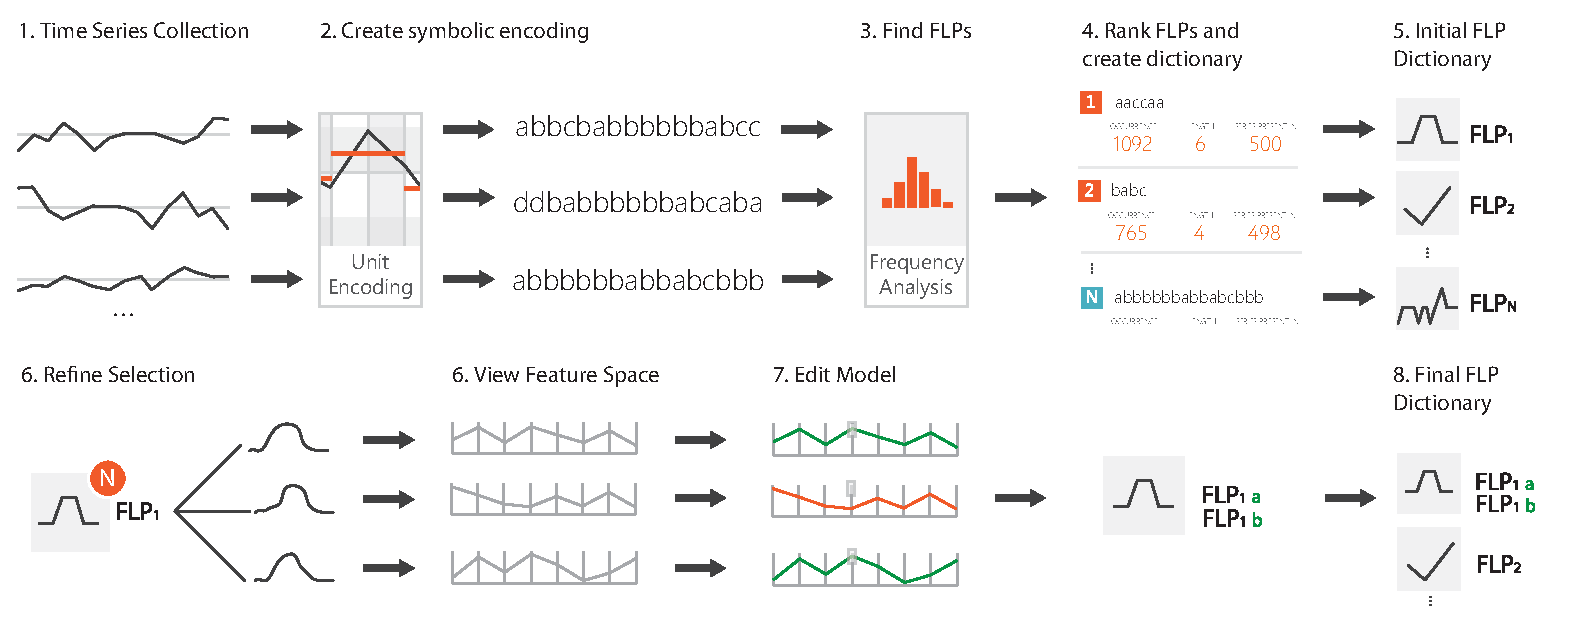
\includegraphics[width=\textwidth]{images/timeseries/overview.pdf}
\caption{Dictionary compilation steps -- given a number of time series datasets ($T_1, T_2, \ldots, T_n$) (1), each is approximated by a symbolic representation (2). A list of Frequent Long Patterns (FLPs) are found (3) from analysis of the symbolic encodings and these FLPs are ranked by their ``compression potential'' (4). Highly-ranked FLPs are added to an initial dictionary. Each FLP mdoel can be refined at more granular levels by selecting for particular features of the set of time series it represents.
Finally, we have an FLP model dictionary.}
\label{fig:overview}
\vspace{-10pt}
\end{figure*}

In data compression, \emph{dictionary encoding} is a family of methods that search a text for strings from a dictionary, and replace the matching strings with the corresponding codewords defined in the dictionary.
The same dictionary is maintained by the encoder and the decoder, facilitating faithful translation from the original text to the compressed representation, and back to the original text. 
The primary goal of such a compression strategy is to reduce storage requirements.
In a less algorithmic form, we apply a similar approach in writing by using abbreviations (\eg, UN for United Nations and symbols (\eg, \textsection~and \textcopyright)).
Such a compression method can be based on:
a general dictionary applicable in a wide context (\eg, commonly-used currency signs);
a dictionary that is meaningful only to a specific group of people or in a specific context (\eg, mathematical symbols, abbreviations for measurement units);
or an \emph{ad hoc} dictionary to address a very specific requirement (\eg, we introduced FLP as an abbreviation for \emph{Frequent Long Pattern}).
The primary goal is to reduce the time and cognitive load required for reading long and frequently-occurring text strings, while it also facilitates space saving in many cases.

The condition of \emph{long} and \emph{frequently occurring} reflects the principle of \emph{entropy encoding} in information theory \cite{Chen10}.
The most well-known entropy encoding technique is Huffman coding.
In everyday life, we can observe many intuitive entropy encoding schemes.
For example, traffic signs are designed to speed up readings of restrictions and instructions, which otherwise would require a few words or sentences.
For less commonly used restrictions and instructions, we still have text-based traffic sign boards.
The balance between icon- or glyph-based and text-based visual representations in traffic signage features considerations of frequency of usage, length and complexity of the original text, importance, and various human factors (\eg, learnability, recognition, and memorisation).

This has inspired us to apply the concepts of entropy encoding and dictionary encoding to visualization, since they are everyday phenomena that are underpinned by well-established mathematical theories.
We can draw a parallel between a time series and a piece of text, and between a frequent long pattern in a collection of historical time series and a common long string in a text corpus.
This analogy suggests that we can adopt a computational process to compile a dictionary, since  there have been many previous works on symbolic processing of time series data in the literature (\eg, \cite{lin2005}).
As glyphs have been used for time series visualization (\eg, \cite{Saraiya2005}), we thus focus on a visual representation that supports dictionary-based compression while maintaining overview and selective detail views.


Figure \ref{fig:overview} illustrates the algorithmic steps for creating the FLP dictionary for a corpus of times series data.
This dictionary creation algorithm is designed to process a collection of time series in order to establish a dictionary consisting of a set of FLPs in a specific context, and consists of the following steps:

\begin{enumerate}
\item\textbf{Time Series Collection.}
It is necessary to collect a set of time series in order to generate good statistical indications about common patterns and outliers;
\item\textbf{Unit Encoding.}
Given a collection of time series, the next step in \emph{Dictionary Compilation} is to translate them to symbolic representations.
These symbolic representations collectively form a text corpus;
\item\textbf{Find FLPs.} In this step, an efficient algorithm based on a suffix tree structure is deployed to detect a list of FLPs;
\item\textbf{Ranking FLPs.} For each detected FLP, we compute its potential compression capacity alongside other parameters in the feature space (see Section \ref{sec:feature_space}). We then choose the high capacity patterns and/or those with features matching any user-defined requirements defined in the visual analytics platform; and
\item\textbf{Creating Glyphs.} The glyphs can be created automatically based on various attributes of the time series they represent.
\end{enumerate}
%
%Consider that we have $N_p$ FLPs in a time series, and each FLP is of a length of $M_i (i=1, 2, \ldots, N_p)$ samples.
%If each glyph requires a display space with a fixed width $\omega_g$ (in pixels), the compression ratio in terms of horizontal visual space requirement is:
%
%\begin{equation}
%\label{eq:PatternRatio}
%	C_{FLPs} = \frac{\omega_s \sum_{i=1}^k M_i}{\omega_g N_p}
%\end{equation}
%
%\noindent where $\omega_s$ is the number pixels per sample, including interval space, along the $t$-axis in a conventional line graph.
%The overall compression ratio for the time series is
%
%\begin{equation}
%\label{eq:SeriesRatio}
%	C_{timeseries} = \frac{\omega_s N_t}{\omega_s (n - \sum_{i=1}^k M_i) + \omega_g N_p}
%\end{equation}
%
%Spatial compression is merely an indicator of the potential benefits of a frequency-based encoding strategy. 
%In general, representing parts of a time-series as appropriate glyphs can benefit some common visualization tasks, such as identifying familiar FLPs, focusing attention on potential anomalies, and performing visual searches.
%The main cost is the loss of accuracy of those glyph-encoded parts of the time series.
%The trade-off is a universal mechanism at the heart of visualization.
%Many visualization techniques, such as zooming, glyph-based techniques, and metro-maps, feature such a trade-off.
%In fact, the conventional line graphs for time-series visualization usually incur a significant loss of accuracy in comparison with the raw data, since the screen resolution is usually much lower than the data resolution.
%With interactive visualization, the loss of accuracy in overview can be recovered from details on demand \cite{shneiderman96}, for example, using zoom or pop-up windows.

%\item\textbf{Dictionary-based compression}
%\begin{enumerate}
%\item\textbf{Deployment.} The dictionary is now ready to be deployed to process newly arrived time series.
%\item\textbf{Unit Encoding.} For an input time series, we first translate it into a symbolic representation.
%\item\textbf{Finding FLPs.} We then search for all FLPs in the text string based on the dictionary.
%\item\textbf{Glyph-encoding.} The corresponding glyphs are attached to the data structure of the time series.
%\item\textbf{Glyph-based visualization.} The time series is visualised with the support of glyph-based abstraction, continuing overview, integrated detail views for less common patterns, and further details on demand for FLPs.
%\end{enumerate}
%\end{itemize}

\subsection{Unit Encoding}
\label{sec:Unit}
Let $T$ be a time series with $N_t$ samples.
We first divide it into $N_{unit}$ \emph{time units}, each of which consists of a fixed number of samples ($N_{spu}$) such that
$N_{unit} = \lceil N_t / N_{spu} \rceil$.
In the literature, various terms have been used to denote such a time unit, e.g., `time primitive' and `chronon' in \cite{markus13} and `window' in \cite{lin2005}.

An encoding scheme is then selected to map each unit to a symbol in an alphabet $A$.
In this work, we chose to base our algorithm on the symbolic approximation (SAX) approach since it:
1) is widely used by the time series community;
2) is performant with O(n) complexity; and
3) has output ideally formed for indexing, hashing and storage in data structures such as suffix trees as performed in \cite{lin2005}. 

This approach takes the mean of the values within a window, then assigns a character to that mean depending on where the value falls in the gaussian distribution calculated using Z-normalisation.
The potential compression ratio is influenced by the size of the alphabet $|A|$, and the number of samples per unit $N_{spu}$.

Additionally, the unit encoding algorithm provides an option to compress the series before running the FLP detection algorithm.
This compression step encodes the run length of a particular sequence as a single number, and can result in more general FLPs that accommodate many more series that have the same shape/profile but different lengths.
Our compression technique works by taking a symbolic approximation, say \emph{aaaaaaabccccbbb} and translates this to \emph{a3b1c2b2}. All short sequences ($\le 3$) map to $1$, medium sequences ($3 < x \le 7$) map to $2$, and long sequences ($>7$) are mapped to $3$.

\subsection{Frequent Long Pattern (FLP) Detection Algorithm}
\label{sec:FLP}

From the symbolic representation calculated in Section \ref{sec:Unit}, we need to extract the most common, long substrings from an available set of sequences with the expectation that selection of the most common strings will lead to greater compression. 

The FLP detection model has three principle components: an enhanced suffix array (with longest common (LCP) prefix array) to provide a fast, space efficient platform for fast string searching; an algorithm to compute the common elements in the string and their frequency; and a filter to fulfil any user-defined refinements on the features that motifs should have - by default, the model satisfies the requirement of finding those patterns matching the FLP properties of both \emph{long} and \emph{frequent}.

\subsubsection{Finding the FLP Candidates}
\label{sec:Find}

\begin{figure}[!t]
\centering
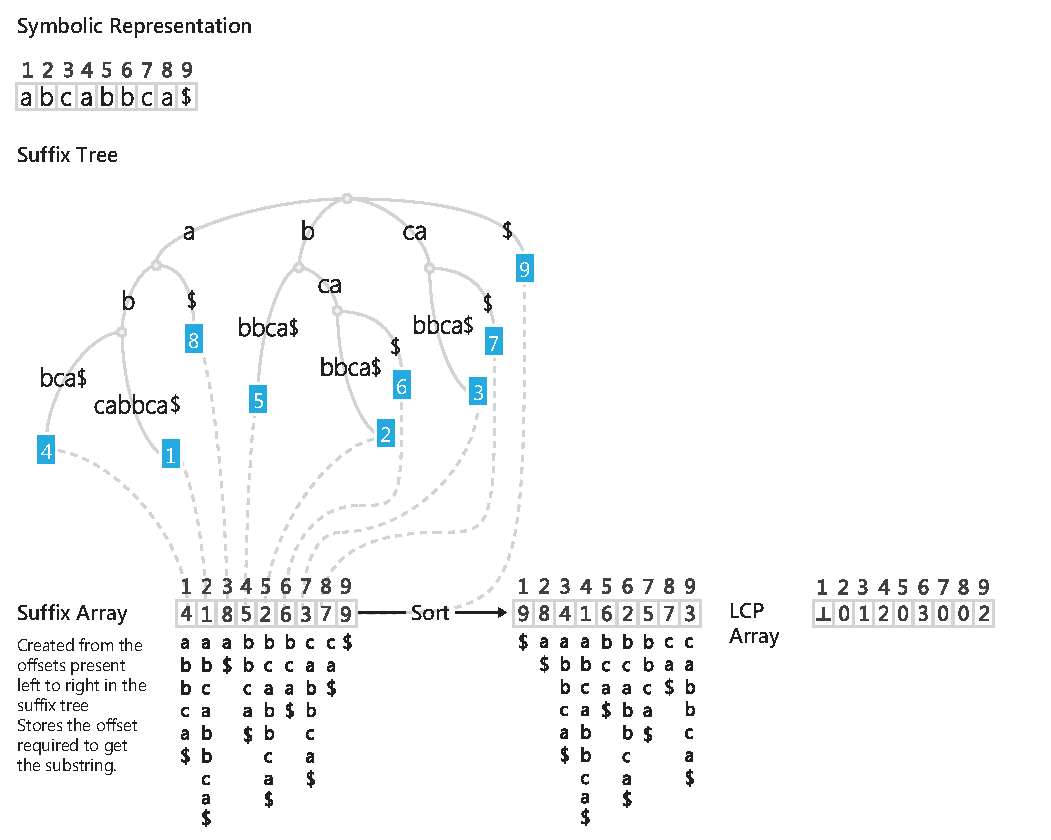
\includegraphics[width=\textwidth]{images/timeseries/suffix_tree.pdf}
\caption{A suffix tree, suffix array, and longest common prefix (LCP) representation of a string \emph{``abcabbca''}.
The \$ symbol indicates the end of a string.}
\label{fig:suffix_tree}
\vspace{-10pt}
\end{figure}

The suffix tree (or position tree) was first defined by Weiner in 1973 \cite{weiner1973}.
It is used to represent all possible suffixes (endings) of a string \cite{weiner1973, ukkonen1995}.
Figure \ref{fig:suffix_tree} presents an example of such a tree and its corresponding suffix and longest common prefix (LCP) arrays \cite{kasai2001}.
Suffix trees thrive in their ability to speed up previously computationally intensive string operations such as: finding the longest common substring; finding repeats; finding maximal palindromes; and inexact string matching (the Weeder algorithm). 

While suffix trees are fast to query and build, they are costly to store.
An alternative to the suffix tree is the suffix array, a sorted array of all suffixes.
Using the suffix array, it is possible to perform all tasks that a suffix tree can perform in the same time when 'enhanced' with a Longest Common Prefix (LCP) array \cite{kasai2001, abouelhoda2004}.
The LCP array gives for each adjacent pair of suffixes, the longest common prefix shared between them.
For example, as shown in Figure \ref{fig:suffix_tree} the longest common prefix between the suffixes at positions five ``\emph{\textbf{bca}}'' and six ``\emph{\textbf{bca}bbca}'' is three, referring to the length of ``\emph{bca}'' common to both.

The algorithm below finds ``non-gapped motifs'' that were first formally defined by Esko Ukkonen \cite{ukkonen2007structural}).
This algorithm takes a collection of time series approximations $S_{approx}$, finds all the common patterns, then returns a filtered list of FLPs matching the criteria defined in Section \ref{sec:bestFLP}.

\begin{algorithm}
\caption{FLP Detection Algorithm}
\begin{algorithmic}[1]
\Function{Detect\_FLPs}{$S_{approx}$}
	\State $Set_{FLPs} \gets \{\}$
	\ForAll{$S_{i} \in S_{approx}$}
		\State $Array_{suffix} \gets \textbf{sort}(\textbf{createSuffixArray} (S_{i} ) )$
		\State $Array_{lcp} \gets \textbf{createLCPArray}(Array_{suffix})$
	
		\State $pos_1 \gets 0$
		\State $index \gets 0$	
	
		\While{$index < Array_{lcp}.length$}
			\State $pos_2 \gets Array_{suffix}[index+1]$			
			\State $length \gets Array_{lcp}[index]$		
			\State $end_{index} \gets \textbf{max}(pos1, pos2) + length$			
			\State $FLP_{candidate} \gets $\textbf{getSuffix}($S_{i}, index, end_{index}$)			
		\If{$FLP_{candidate} \exists Set_{FLPs}$}
			\State \textbf{get}($Set_{FLPs},FLP_{candidate}$)$.occurrence$++			
		\Else
			\State $FLP_{candidate}.occurrence \gets 1$
			\State $Set_{FLPs} \gets FLP_{candidate}$
		\EndIf
			\State $index \gets index+1$
			\State $pos1 \gets pos2$
		\EndWhile
	\EndFor
 	
	\Return \textbf{Filter\_FLPS}($Set_{FLPs}$) \Comment{see \ref{sec:bestFLP}}

\EndFunction
\end{algorithmic}
\label{alg:FLP}
\end{algorithm}

\subsubsection{Selecting the ``Best'' FLPs}
\label{sec:bestFLP}

Let $\Xi$ be an FLP found using the detection algorithm in Section \ref{sec:Find}, which can be written as a series of letters $\Xi = \alpha_1\alpha_2\ldots\alpha_m$.
$L_{\Xi}$ denotes its length (\emph{i.e.}, the number of letters) and $F_\Xi$ denotes its frequency of occurrence obtained by the detection algorithm.
$F_\Xi$ can be the number of occurrences of $\Xi$ in the data repository, or be moderated by a predefined maximum number.
The compression ratio for $\Xi$ is
% 
\begin{equation}
	\label{eq:FLP_compression}
	C(\Xi) = \frac{\omega_s \times N_{spu} \times L_{\Xi}}{\omega_g}\\
\end{equation}
%
\noindent In Equation (\ref{eq:FLP_compression}), $\omega_s$ is the minimal width along the $t$-axis required to adequately distinguish a data point in a time series (\eg, 2 pixels), $\omega_g$ is the screen width of a glyph, and $N_{spu}$ is the window size for the symbolic approximation (\emph{i.e.}, the number of samples per letter).
As the actual realisation of this compression ratio depends on the probability of its occurrence in an input string, we moderate $C(\Xi)$ with $F_\Xi$ as
%
\begin{equation}
	\label{eq:potential_compression}
	P_C(\Xi) = F_\Xi \times C(\Xi)
\end{equation}

We refer to $P_C(\Xi)$ as the \emph{potential compression power} of $\Xi$.
For example, consider a 20-letter string and $\Xi$, $N_{spu} = 10$.
This FLP has 200 samples.
If $\omega_s$ = 2 pixels, and $\omega_g$ = 40 pixels, we have $C(\Xi) = \frac{2 \times 10 \times 20}{40} = 10$.
This implies that the glyph replacement will take up 10\% of the original space requirement for the 200 samples.
Assuming an unmoderated $F_\Xi = 50$, we have $P_C(\Xi) = 500$.

The key balance to be found in the approach is finding the optimal number for $N_{spu}$ for any given dataset so that the system is able to compress optimally and intelligently.
A larger number for $N_{spu}$ will lead to a coarser representation of the time series, however it will probabilistically lead to further rates of compression. Conversely, a small number for $N_{spu}$ will result in a more fine grained approximation for all time series but lead to less compression due to a generally higher amount of entropy in the approximation.

The selection of $N_{glyphs}$ ``best'' FLPs relies mainly on the $P_C$ scores.
This may depend on a predefined limit of $N_{glyphs}$, as too many glyphs would incur extra difficulties in learning, recognition and memorisation.
This may alternatively depend on a preset threshold for $P_C$.
In the simplest case, the process can stop here and the results can be compiled into a dictionary of FLPs $\mathcal{D}$. The resulting dictionary can then be used to compress a time series (see Section \ref{sec:vis_results}).

In some cases however, an FLP may classify what can be deemed an anomaly along with normal patterns due to subtle differences in the series even though the overall shape of the distribution is similar. This is where the visual analytics platform comes in to play whereby users can view the feature space of an FLP (mean, standard deviation, kurtosis, etc.) can sub classify an FLP and its corresponding time series with more fine-grained control.

\section{Feature Space}
\label{sec:feature_space}

%Given the FLPs (Frequent Long Patterns) returned from the FLP detection algorithm, basic glyphs can be created based on the symbolic approximation. 
%Figure \ref{fig:glyph-design} illustrates the design of a glyph for representing a FLP in a time series to be compressed.
%Such a glyph may encode many different types of information related to the FLP, and the corresponding section of the time series to be compressed.
As mentioned earlier, the FLP detection subsystem in Section \ref{sec:flp_detection_model} focuses on noise tolerance. Each of the selected FLPs determines an individualised model, $\Xi$.
This represents a significant approximation in terms of both temporal range and attribute value range.
A selected FLP can easily encompass many similar patterns of the time series.
To be able to distinguish between those time series segments that are valid versus those that are not, we need the visual analytics platform to refine the model.
First, we apply the individualised model, $\Xi$, to all or a subset of time series in the corpus. This would result in a collection of results,
$\mathcal{R} = \{R_1, R_2, \ldots, R_m\}$, detected by using $\Xi$.
We then construct a feature space for $\mathcal{R}$.

There are a variety of computable attributes for time series data used in the literature (\eg, twenty three considered by Tam \etal \cite{tam2011}). We consider a number of these variables to characterise each motif and the times series data they represent.  

Alongside more trivial metrics such as \emph{maximum} and \emph{minimum} values, \emph{average}, \emph{standard deviation} and \emph{variance}, the software also calculates the following:
%This selection of specific types of attributes for glyph encoding will depend on application needs.
%In this work, we select the following attributes to demonstrate the process.
%
%\begin{enumerate}
%\item \emph{Time series approximation}: this approximation is given by the unit encoding algorithm and provides an overview of what the represented time series looks like;
%\item \emph{Run length}: the run length shows how long this pattern has appeared for in the series and is key to enabling compression of the series, collapsing many similar glyphs into one; 
%\item \emph{Continuity}: this concerns how the glyph will integrate with the actual time-series in the final compressed representation. The strategy taken, and illustrated in Figure \ref{fig:glyph-design}B is to make the height of the time series and approximation area within the glyph the same height; and
%\item \emph{Statistics}: for the purposes of this work, we identified four metrics, a subset of which can be used for annotation of each time series glyph: 
\begin{enumerate}
\item \emph{Correlation/error}: calculated as the Pearson product-moment correlation coefficient between the approximation values and the original time series values as a way of identifying how close the approximation is to the reality. This coefficient is defined in Equation \ref{eq:correlation} where $X$ and $Y$ are two arrays representing the approximated series and the time series respectively, and $\bar{X},\bar{Y}$ represent the mean of both arrays.

\begin{equation}
\label{eq:correlation}
	\rho = \frac{\sum_{i=1}^n (X_i - \bar{X})(Y_i - \bar{Y})}{\sqrt{\sum_{i=1}^n (X_i - \bar{X})^2}\sqrt{\sum_{i=1}^n (Y_i - \bar{Y})^2}}
\end{equation}

\item \emph{Kurtosis}: kurtosis, as illustrated in Figure \ref{fig:glyph_design_features} gives a measure of the peakedness of a distribution.
This is calculated using the equation defined in Equation \ref{eq:kurtosis} where $X$ is the original time series $T$.


\begin{equation}
\label{eq:kurtosis}
	\kappa = \frac{1}{n\sigma_{X}^4} \sum_{i=1}^n (X_i - \bar{X})^4
\end{equation}


\item \emph{Skewness}: the skewness, illustrated in Figure \ref{fig:glyph_design_features} gives a measure of curve asymmetry and is defined in Equation \ref{eq:skewness}.

\begin{equation}
\label{eq:skewness}
	\gamma = \frac{1}{n\sigma_{X}^3} \sum_{i=1}^n (X_i - \bar{X})^3
\end{equation}

\item \emph{Burstiness}: also called local variance, indicates how quick adjacent values rise or fall. The equation below has been adapted from Shinomoto \etal \cite{shinomoto2003differences}. 

\begin{equation}
\label{eq:local_variance}
L_V= \frac{1}{n-1}  \sum_{i=1}^{n-1} \frac{3(X_i - X_{i+1})^2}{(X_i + X_{i+1})^2}
\end{equation}

\end{enumerate}

Additionally, each motif has a compression potential calculated as part of the FLP algorithm discussed in Section \ref{sec:FLP}.

Similar to Tam \emph{et al} \cite{tam2011}, we visualise these parameters using parallel coordinate plots (see Figure \ref{fig:analytics_environment}D) and provide interaction to allow users to edit the model.
Additionally, these features can be incorporated in to glyphs as illustrated in Figure \ref{fig:glyph_design_features} and visualised for the user.

\begin{figure}[t!]
\centering
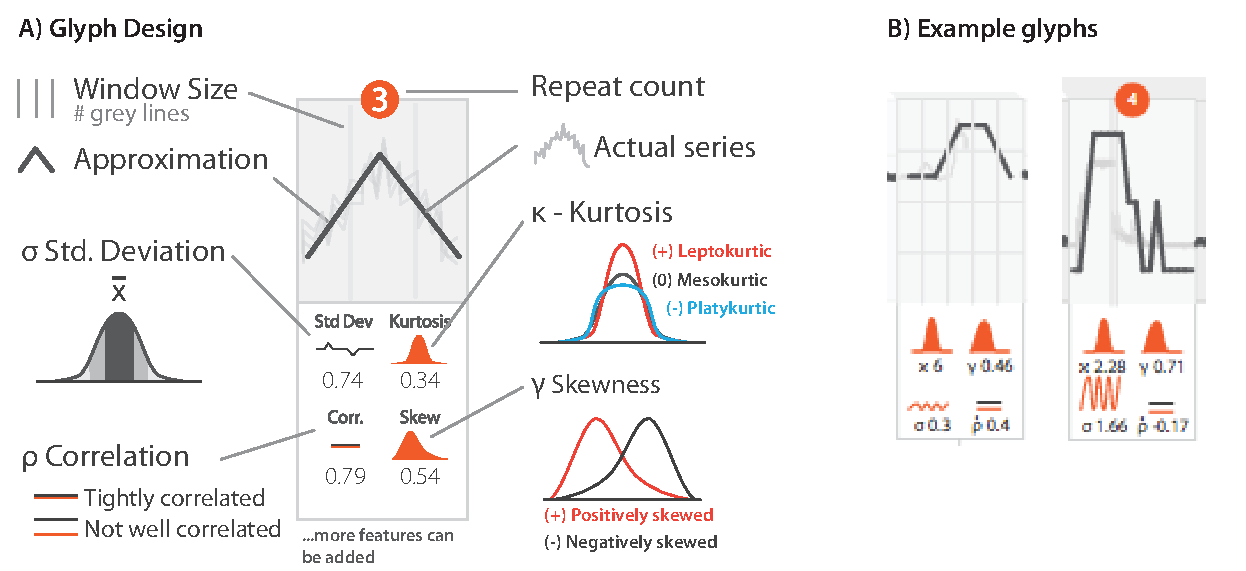
\includegraphics[width=\textwidth]{images/timeseries/glyphs_feature_space}
\caption{A) The time-series glyph encodes eight parameters, four of which are mandatory.
The top half encodes information about the time series profile including: the window size; the approximation of the time series calculated using the SAX approach; the actual profile of the series that made up the profile; and the repeat size (how many times this same pattern has been repeated). The bottom half of the glyph can be configured to show or hide the most appropriate metrics to describe the time series.
Here, the standard deviation, correlation, kurtosis and skewness metrics are presented. B) Some example glyphs from the implementation.}
\label{fig:glyph_design_features}
\end{figure}

%Depending on the application domain, the additional information presented on these glyphs could be changed. For example, if visualising patient cardiac data via ECG, it would be useful to have more domain specific visual encodings to aid the practitioner further in their diagnosis.

\section{Model Editing}
\label{sec:model_editing}

\begin{figure*}[ht!]
\centering
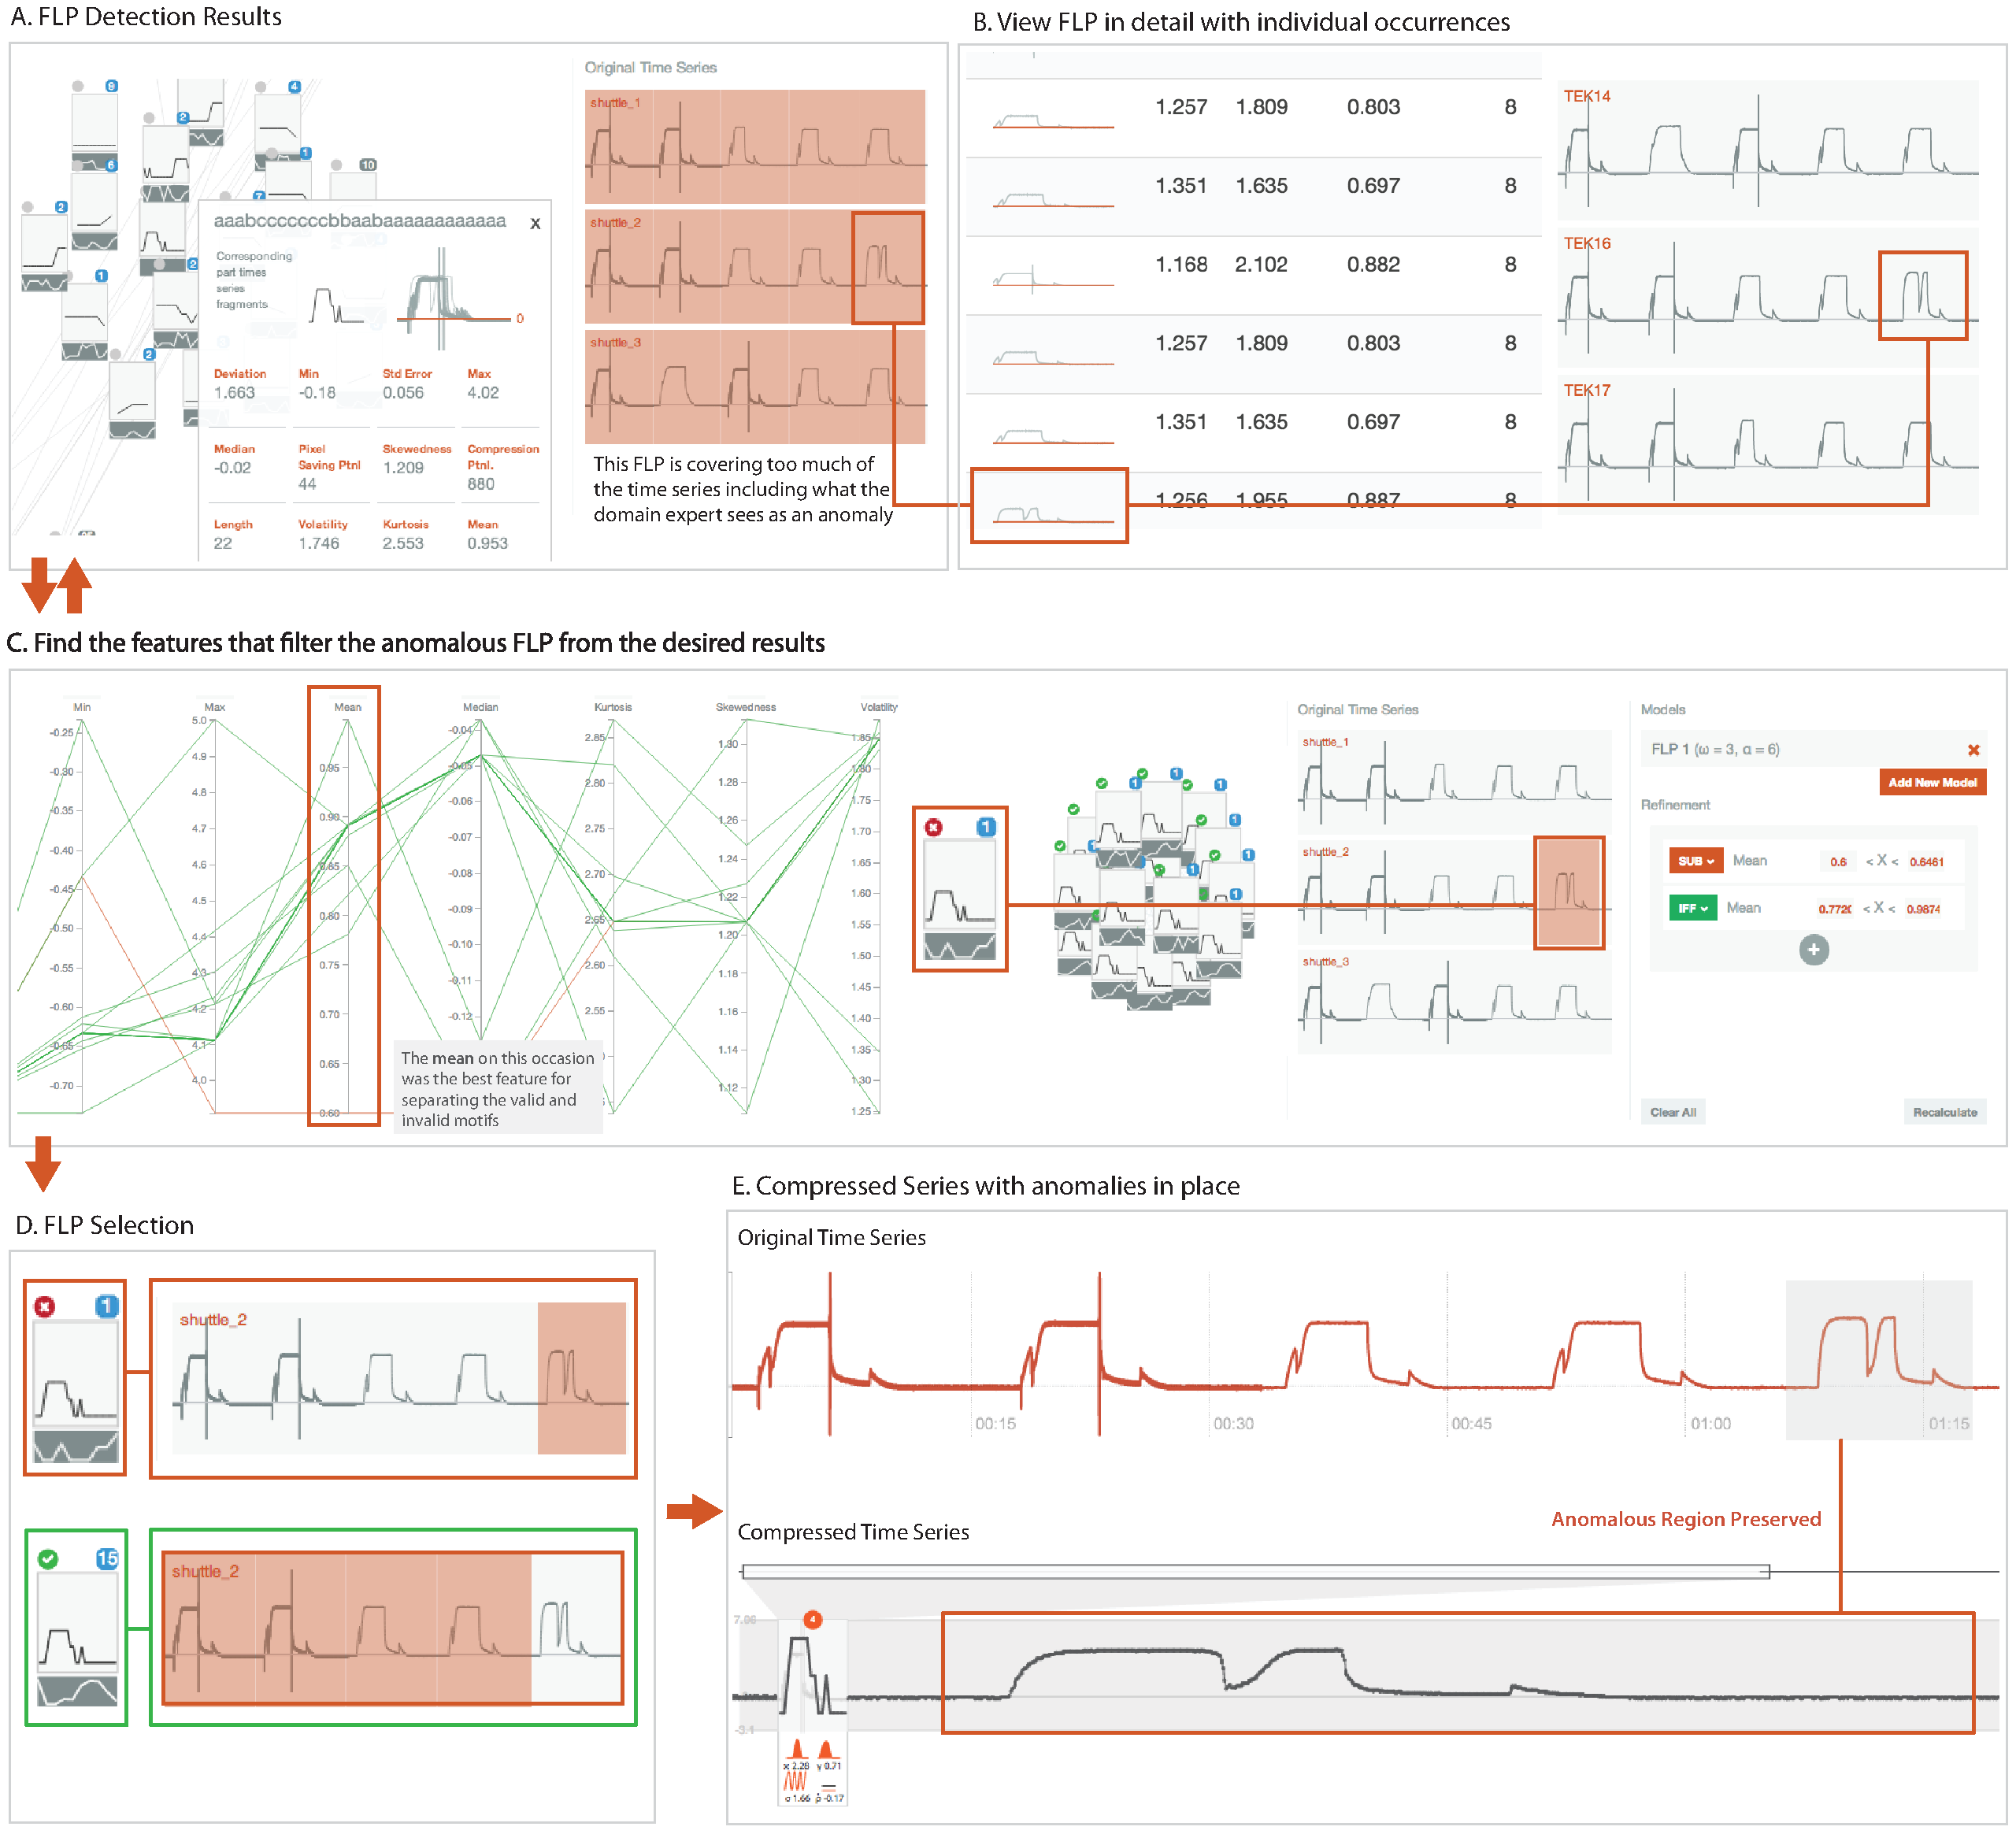
\includegraphics[width=\textwidth]{images/timeseries/results}
\caption{A visual analytics approach to model refinement on an engineering time series dataset depicting the solenoid current measurements on a Marotta valve used to control fuel on a space shuttle from benchmarking datasets by Keogh \etal \cite{shuttle_data}. This dataset was used since ground truth was known. By finding the given anomalies, we were able to validate our work.}
\label{fig:results}
\end{figure*}
%
%\begin{figure*}[ht!]
%\centering
%\includegraphics[width=\textwidth]{images/timeseries/result_ecg}
%\caption{The same visual analytics approach to model refinement on an electrocardiogram dataset from benchmarking datasets by Keogh \etal \cite{shuttle_data}.}
%\label{fig:results_ecg}
%\end{figure*}

Model editing is supported through a dedicated user interface within the visual analytics platform. 
This functionality is demonstrated through an example in Figure \ref{fig:results} where the motif-finding algorithm is applied to a time-series data from algorithm benchmarking datasets from Keogh \etal \cite{shuttle_data}. 
This dataset contains solenoid current measurements on a Marotta valve used for fuel control on a space shuttle.

In Figure \ref{fig:results} A, a network view displays the motifs found by the FLP detection algorithm as glyphs. 
Hovering over a glyph highlights the original time series values that glyph represents in orange. 
Expert-derived annotations however pointed to an anomaly which the motif-finding algorithm had grouped with the ``normal''  profiles. 
This FLP is highlighted in the black outline. 
The next step will involve filtering this pattern out by looking in more detail at the FLPs, the time series patterns they represent, and their feature space. 

Figure \ref{fig:results} B shows a view of all 16 occurrences of the FLP of interest from the first step. 
Each occurrence of a motif is now represented by its own node in the network graph. 
Additionally, each node has its own feature space. 
Through clicking on the motif of interest one can see that the time series profile matches the anomalous series we wish to exclude.

Having identified the anomalous motif, Figure \ref{fig:results} C shows how, through use of the parallel coordinates, we can find the features that are able to classify between the valid and invalid FLPs. 
In this case, the mean was a good choice since the anomalous FLP had a mean much lower than the others (likely to be caused by the significant dip in the middle of the profile). 
The network layout automatically updates to visually separate the rejected FLPs from those that were accepted. 
Figure \ref{fig:results} D, shows the resulting FLPs which are then exported as a dictionary along with feature refinements (\eg the \emph{mean} filter) for later compression. 
Finally, Figure \ref{fig:results} E shows a time series $T$ compressed using the FLPs in the dictionary. 
The result is a compressed representation of the time series with the anomalous region preserved. 
This visual compression step is described more in Section \ref{sec:vis_results}.
 
\section{Visualizing the Compressed Time Series}
\label{sec:vis_results}

\begin{figure*}[t!]
\centering
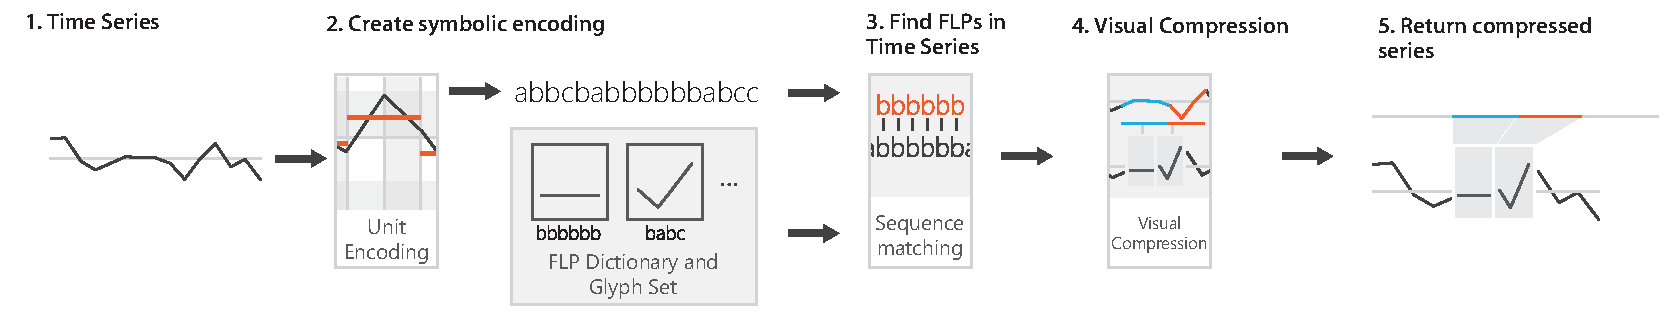
\includegraphics[width=\textwidth]{images/timeseries/glyph_creation_workflow}
\caption{Dictionary-based compression steps -- Given a time series $T_1$, we encode it symbolically (2). Then, with the FLP dictionary created in (A), an algorithm finds the occurring FLPs in the incoming sequence (3). These found FLPs are replaced with glyphs (4) and the compressed time series is visualized.}
\label{fig:compression_workflow}
\end{figure*}

Given a dictionary of FLPs $\mathcal{D}$ obtained from the FLP Detection Subsystem (Section \ref{sec:FLP}), the process of glyph-based time series compression, illustrated in Figure \ref{fig:compression_workflow}, can be applied repeatedly to many time series.
Using traffic signage as an analog, once functional and visual representations of different signs have been decided, we can place them in any applicable location.

Glyph-based time series compression involves two steps: 1) given a dictionary of FLPs $\mathcal{D}$ and a time series $T$, create a compressed representation of a time series; and 2) using this representation of the time series, render it. 

\begin{figure}[t!]
\centering
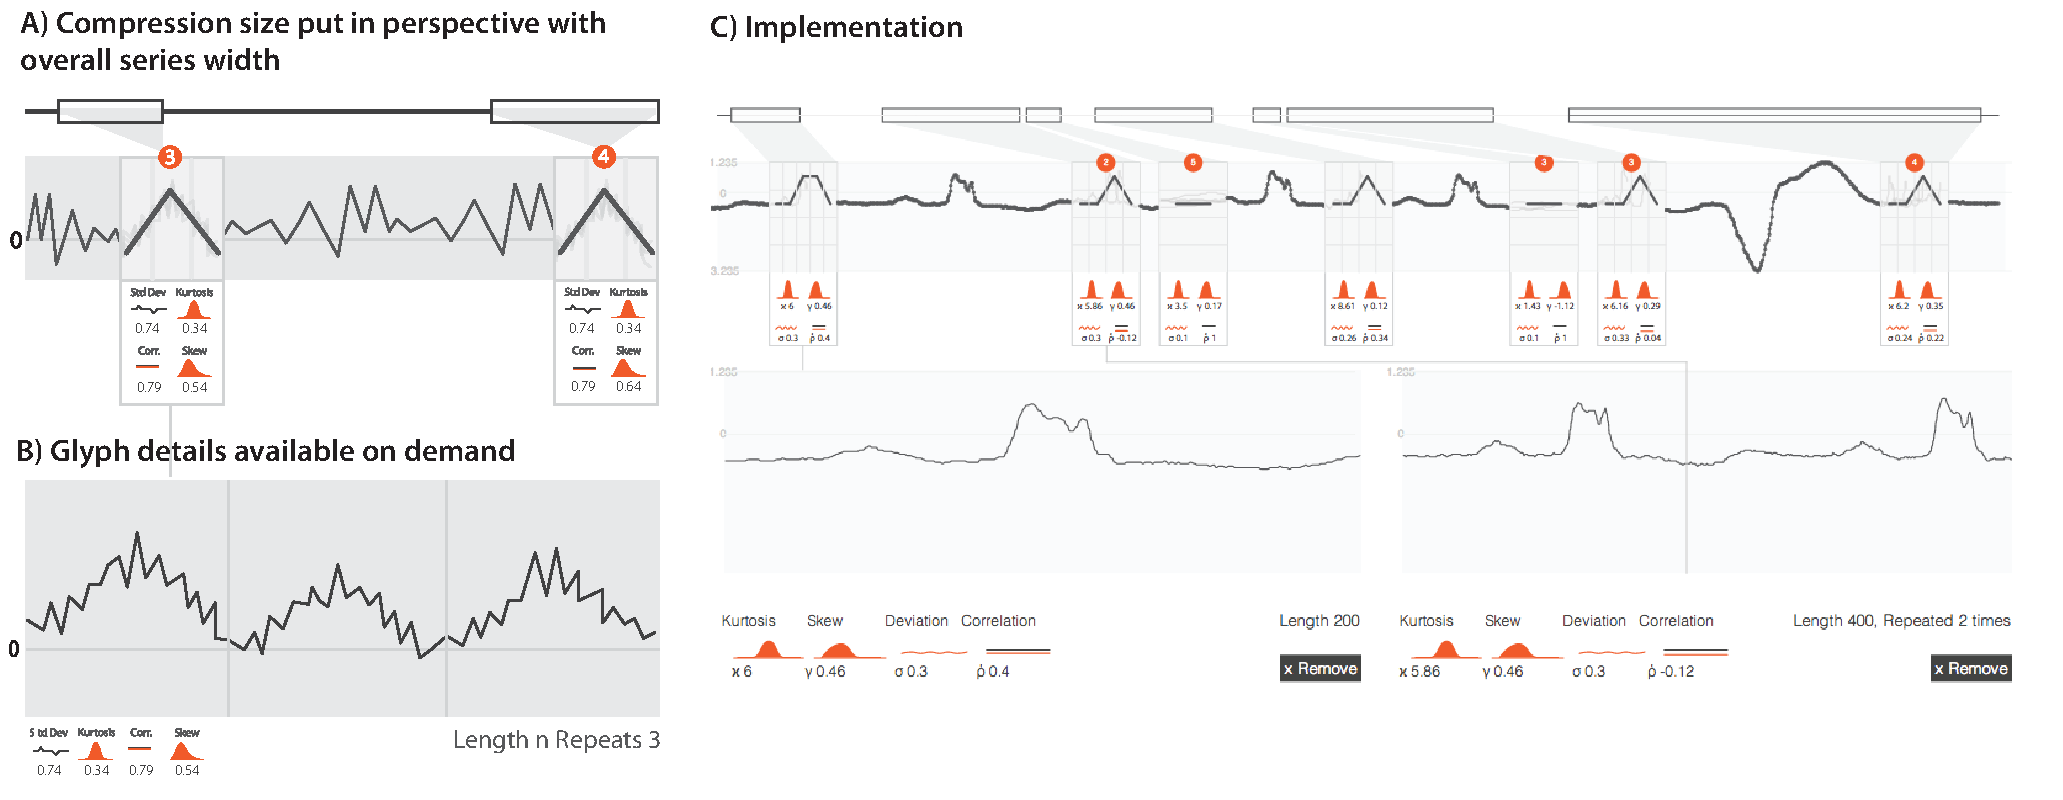
\includegraphics[width=\textwidth]{images/timeseries/glyph_compression_ui}
\caption{A) The compression power of a particular FLP and the part of the time series compressed by a glyph is given by an overview bar. B) Details are available on demand when users click on a glyph in an implementation inspired by StackZooming \cite{javedstack2010}. C) Implementation of the design in A and B showing compression of a respiration dataset.}
\label{fig:glyph_compression_ui}
\end{figure}

For the first step, we create the enhanced suffix array representation as performed when creating $\mathcal{D}$.
From this data structure, a binary search is performed for each of the FLPs defined in $\mathcal{D}$ to identify all positions (defined by the suffix array) the particular FLP appears in.
From the constructed list of matching positions for each FLP, some additional processing is made for the rendering layer.
The first is to merge directly adjacent matches, that is, say one of our FLPs is composed of $abcd$, then for $abcdabcdddd, \ldots$, we have a record of $\Xi_{abcd}\uplus[1,5]$ including a list of matching indexes.
Here the operator $\uplus$ denotes annotation, meaning that a FLP $\Xi$ of symbols $abcd$ is annotated with index values 1 and 5.
Since the distances in the start indexes for the occurrences of $\Xi_{abcd}$ are separated exactly by its length $L_\Xi$,  $1 + L_\Xi = 5$, the second occurrence can be merged with the first, and a repeat count for $\Xi_{abcd}$ is increased, so $\Xi_{abcd}\uplus[{1, R2}]$.
Finally, a further check is performed to ensure that the indexes for the matched FLPs do not overlap, that is if $\Xi_{bcd}\uplus[2,6]$ has start indexes overlapping with $\Xi_{abcd}\uplus[{1,R2}]$. 
In this case, the FLP with the lowest compression ratio ($C$) power will be removed from the results. 
At the end of this process, the software produces a map from each start index of a FLP to its symbolic representation and repeat count. 

The second step, rendering the time series, involves the incorporation of the glyphs representing compressed regions in to a time series visualization, the design of which is shown in Figure \ref{fig:glyph_compression_ui}. 
This representation maintains an overview bar showing the overall length of the time series whilst showing how much of a region has been compressed by a glyph. 
The glyphs provide information about the approximation, the run length (how many times the motif was repeated) and a number of metrics from the feature space. 
Glyphs can be interacted with and expanded to provide details of the underlying compressed time series represented by the glyph. 
This can be seen in Figures \ref{fig:results} A and B. 
Additionally, when large areas are compressed, this changes the rendering of a time series somewhat since the series can spread over a much larger range. 
In many cases this is acceptable, but in some cases, the spacing may introduce interpretation problems. 
To navigate this issue, users can select to maintain the aspect ratio of the original series.


\section{Evaluation}

We performed a number of different evaluations to answer different questions of our system, two based on algorithm performance, the other on software use. 

\subsection{Algorithm Performance}

\begin{figure}[t!]
\centering
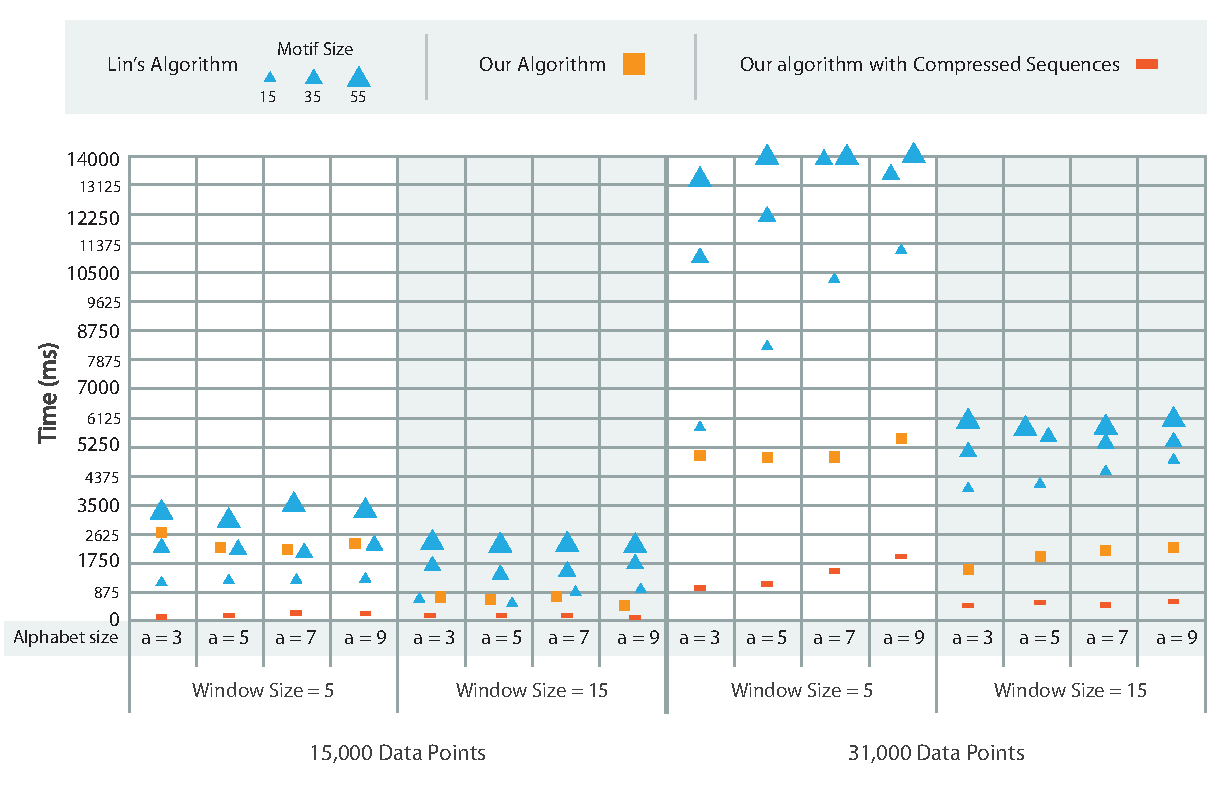
\includegraphics[width=\textwidth]{images/timeseries/benchmarks}
\caption{Analysis of algorithm performance over two different sized data sets with different window (how many data points to be summarised by a letter) and alphabet sizes (how many letters there will be - small values give a coarse approximation, larger values give more granular approximations).
For Lin's algorithm used in VizTree \cite{lin2005}, we also consider different motif size in our comparison since their approach relies on fixed sizes.
For example, a motif size of 15 would mean that there would be 15 letters representing the sequence.
Our algorithm does not need this information and automatically gives back different motif sizes.
This chart shows how the maximum repeat algorithm is considerably faster, especially with larger datasets, however using the maximum repeats algorithm with a compressed sequence representation, we get further performance gains.}
\label{fig:benchmarks}
\vspace{-5pt}
\end{figure}


The closest algorithm to ours that also uses the symbolic approximation approach is that employed by VizTree \cite{lin2005}.
VizTree uses a sliding window algorithm to define motifs of the same length.
Our approach has no restriction on length and simply looks for the patterns that occur most often across sequences.
Not surprisingly, since the sliding window technique is brute force, our algorithm performs quicker across almost all tests, with the difference being substantially larger when data sizes grow.
This is shown in Figure \ref{fig:benchmarks}.

We also tested how our run length compression technique could improve performance.
Since compression will have a normalising effect on sequence length, and as shown in Figure \ref{fig:benchmarks}, sequence length is a major contributor to decreases in performance, we expected performance to improve.
With 35,000 data points, an alphabet size of 3 ([\emph{a, b, c}]), and a window size of 5 (5 data points to one letter), it took 900 milliseconds to analyse the full sequence and detect patterns.
Without compression, this process took 5 seconds, and with the sliding window this took anywhere between 5.6 and 13.4 seconds to complete depending on the size of the sliding window.

What Figure \ref{fig:benchmarks} shows is that the compression-based approach reduces the effects of sequence length, however this technique becomes more sensitive to alphabet size increase.
As the alphabet grows, the heterogeneity of the sequence increases (the entropy is higher).
As a result, compression becomes less effective.
This effect can be counteracted however by increasing the window size.
This has the effect of lowering sequence entropy and increases compression effectiveness.

Additionally, we performed a baseline assessment of algorithm results using publicly available datasets from Keogh \etal \cite{shuttle_data} (to enable reproducibility).
This was performed to test how our algorithm performed on annotated data compared with the existing approach.
Our approach showed a number of benefits.
First, our algorithm reduced the number of motifs by removing repetitive patterns, a consequence of the sliding window technique that identifies patterns using a brute force approach.
Secondly, the motifs that were found were more relevant.
Lastly, our motifs were not restricted by pre-defined segment lengths required by the sliding window algorithm.

\subsection{Interface Performance}

We also assessed our web-based visual analytics software in a number of real-world scenarios including fraud analysis for an online casino software vendor in Oxford, and analyses of penguin count data from the Antarctic with zoologists from the University of Oxford.
Our system was evaluated based on its ability to find the model parameters to create the FLP dictionary for subsequent compression of their time series visualizations.
This was performed by loading their datasets in to the tool and finding the FLPs in their data.
After some initial training, our users from fraud analysis and animal behaviour found the interface intuitive to use, and the results from our algorithm to be more meaningful than those created from the algorithm used in VizTree \cite{lin2005}.

Overall, our analyses showed that our approach is effective at finding the common patterns (and in turn, the anomalous regions of a time series) in a range of time series data for their visual compression.
Our algorithm is performant and the visual analytics support tool has been well received by our initial users.
A video demonstrating the features of the interface is available from \url{http://vimeo.com/120467405}.

\section{Contributions}

The goal of this work was to generate a method for the visual compression of time series plots using a glyph-based approach that follows similar lines to dictionary-based compression approaches.

This approach required the identification of frequent long patterns (FLPs) that would form the eventual dictionary.
To gain a representative view of the data space, so that the resulting FLP dictionary could be used to visually compress other unseen time series from the same domain, our algorithm encourages the input of a time series data corpus.
Such FLP algorithms face a trade off between finding more detailed motifs that do not serve visual compression well, and less detailed motifs that may encompass anomalous regions of the original time series.

To circumvent this problem, a visual analytics approach was used to act as a software development tool to enable users to test the FLP model, analyse, and visualise its results in a feature space (\eg, mean, kurtosis, skewness), identify false positive results, identify related parameter ranges to filter these false positives out, and edit the FLP model accordingly.
This approach allows human users to have the direct control in debugging and refining model results.

Finally, using the resulting FLP dictionary, we provide an interface to visually compress a time series using glyphs that represent FLPs found in the input data.
